\chapter{Results -- Analysis and Performance}

testing took place on a win10 machine, ...
Answer all of the research questions explicitly!!!

-parameter selection gehört hier rein!!

\section{General Performance}

% TODO -dass halt eigentlich zu jedem zeitpunkt compared zu rrt oder human sein müsste

\subsection{Supervised Agents}

-wie schwer es ist die performance von sv-agent zu assessen weil selbst wenn 60\% richtig sind kann das heißen dass er entweder nur geradeaus fährt oder, weil er im ersten frame falsch leigt, noch so viel richtig machen kann und nix davon sieht weil er direkt in die wand fährt
-dass purely pretraining agents nur mit max-speed klappen
-dass nen random agent offensichtlich scheiße ist
-dass man mit supervised agents testen kann ob dataset separable (-dataset is separable as can be tested by dqn\_sv\_agent)
-das headstart scheint helfen
-wie schnell humans fahren
-die beiden offensichtlichen local maxima, erste kurve 16prozent, zweite kurve 30something... wie man sehr deutlich in den plots sieht
-dass ein supervised agent nicht lernen kann da er immer in die wand brettert

\subsection{RL Agents}

-dass alle cars useful driving policies haben: q-werte vor wänden gering, steeren von wänden weg, fahren widely geradeaus... 
-gym\_test klasse existiert, models klappen damit
-mit dem aktuellem reward lernt er das vor der kurve bremsen besser ist als fahren, wie man sieht wenn man davor steht


\section{Incorporating pretraining}

-dass, wenn man actiona slinput gibt, er nur die lernt :o
-dass supervised pretraining nicht übernommen werden kann wegen exorbitanter q-werte
-dass auch q-pretraining nicht funktioniert ohne meinen twist
-dass die ddpg-gaussiandistance-pretraining function nicht funktioniert
-plots von der performance nur pretraining, performance nur ohne, performance nach pretraining einbauen
-dass dqn-models auch leider nicht als base für ddpg taugen, weil sie halt nen output für jede action haben


\section{Discretizing actions}

-plot von ddpg vs dqn

\begin{figure}[h]
%		{%
%			\setlength{\fboxsep}{0pt}%
%			\setlength{\fboxrule}{1pt}%
%			\fbox{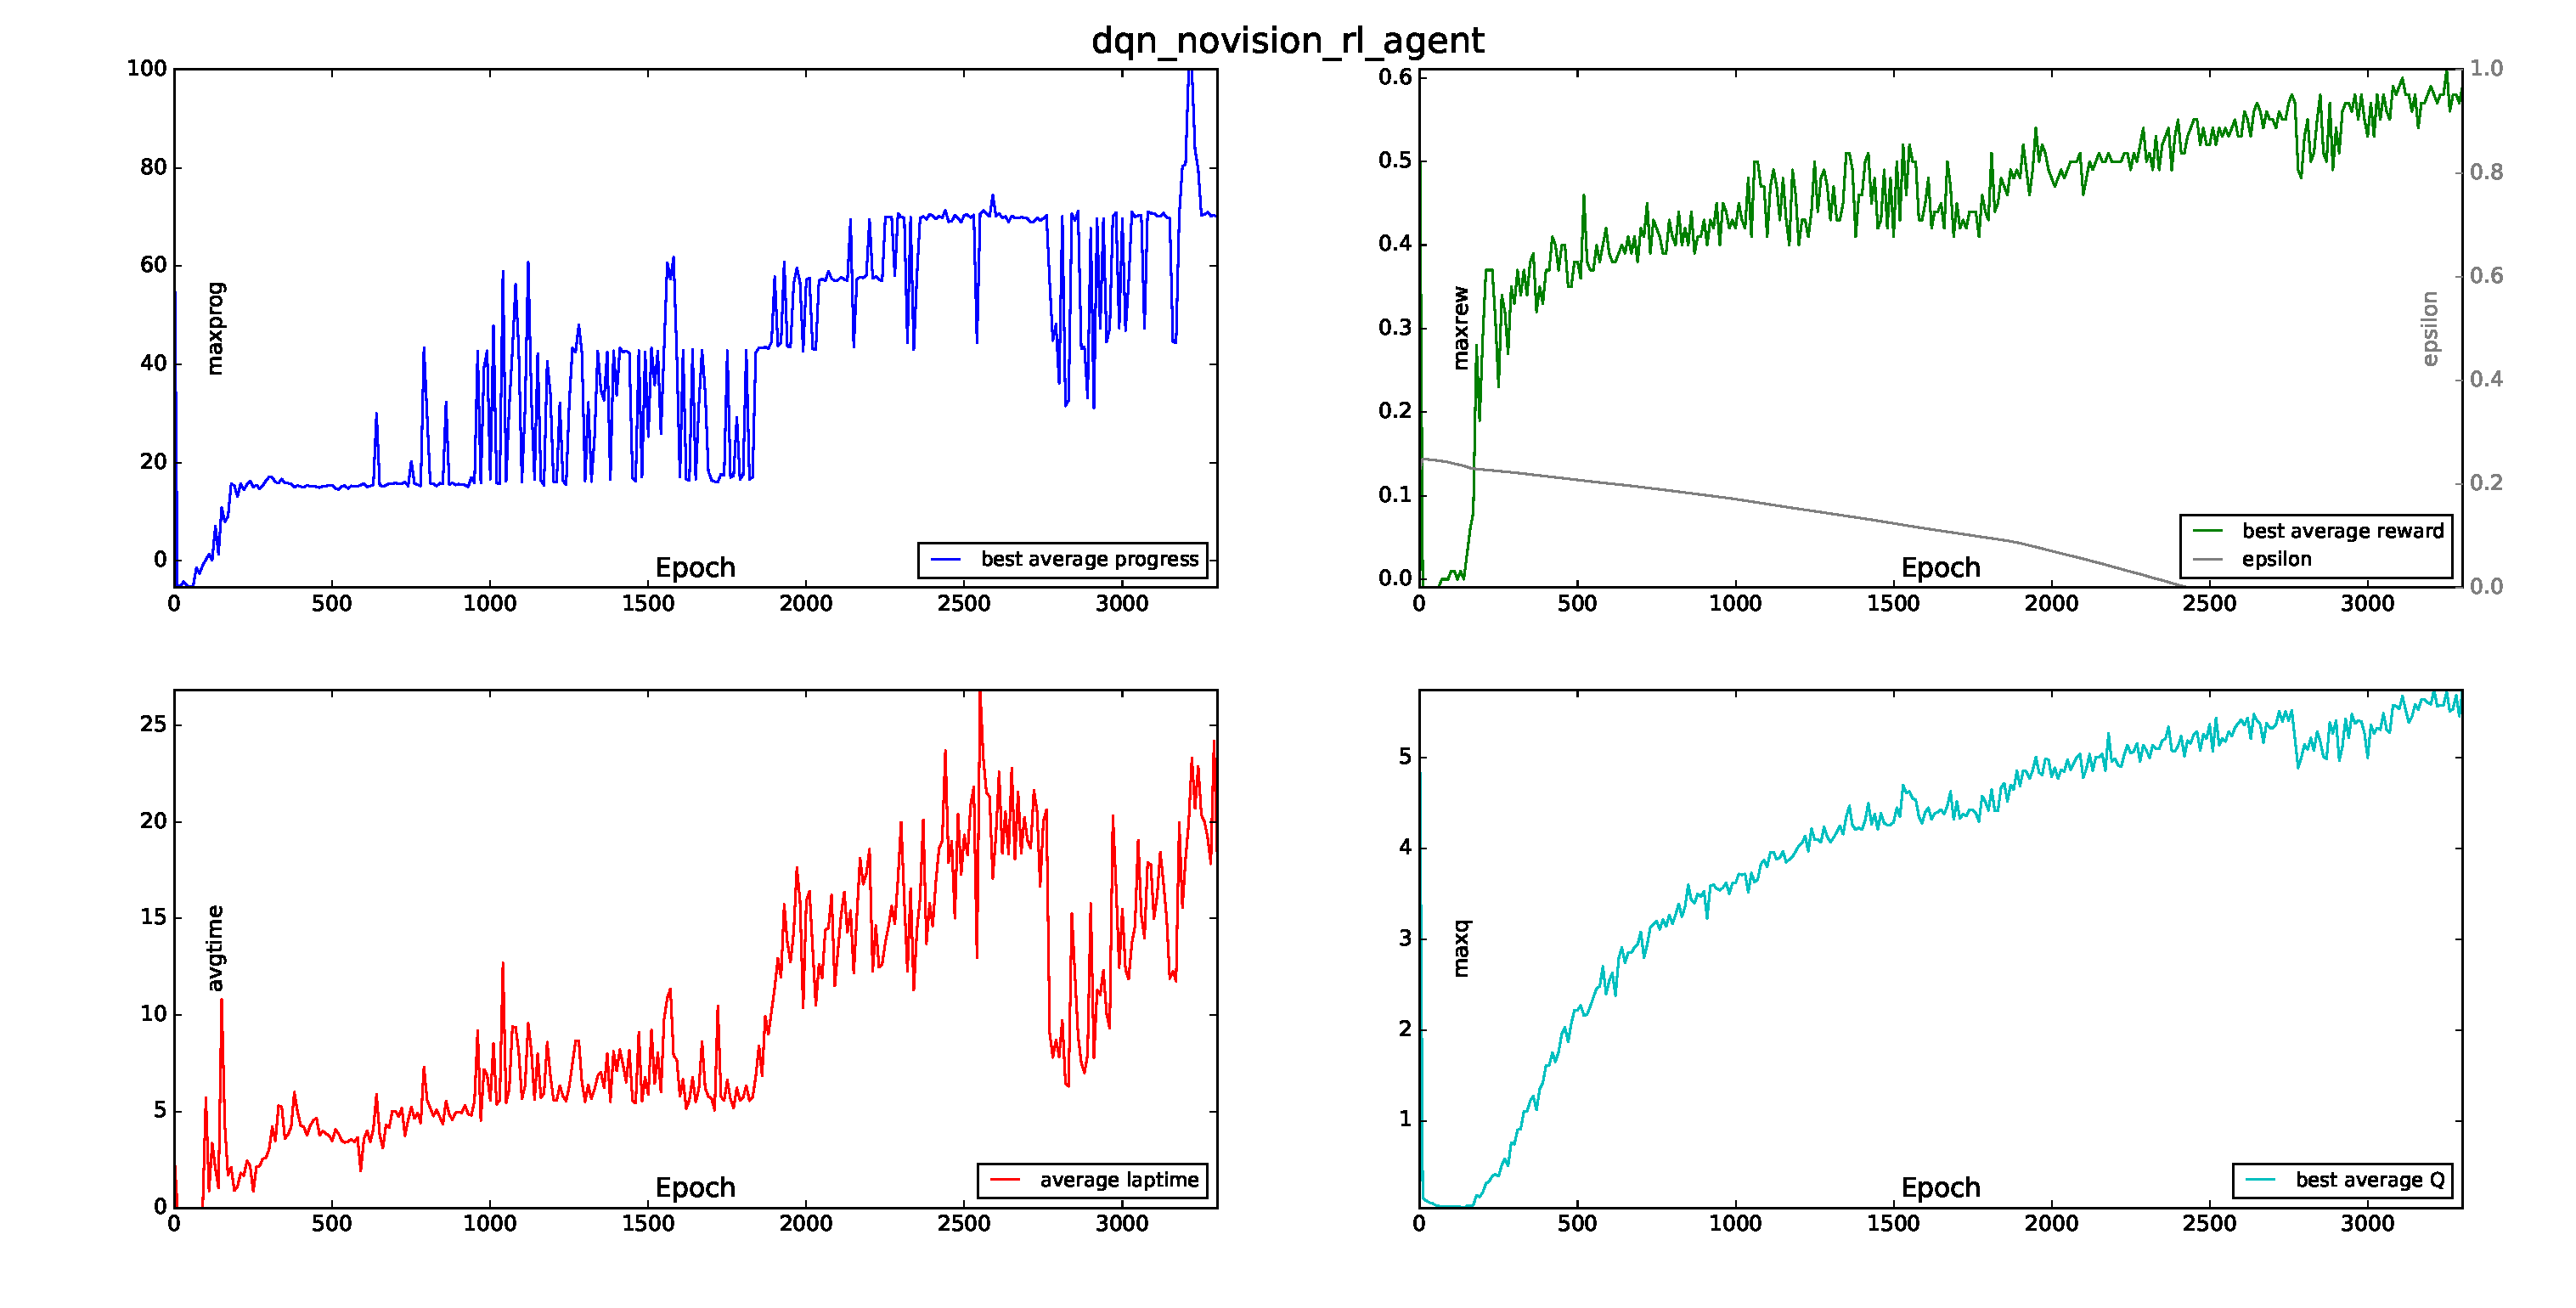
\includegraphics[width=\textwidth]{result_dqn}}%
%		}%
	\colorbox{red}{dazushcreiben dass das mit skript xy gemacht wurde, und die daten dazu online unterxyz zu finden sind, und dass das jeweils der average von 10 runs ist}
	\centering
	\caption{Performance of the dqn\_novison\_rl\_agent}
	\label{fig:dqn_result}
\end{figure}

\section{Reward function}

-meine reward-funktion die bremsen belohnt



\chapter{Discussion and future directions}

\section{Platform}

-dass sich herausgestellt hat das simultaneous inference and learning a lot slower ist!
-die performance vom server
-multiple unity instances (feier-text)
-unity zeit verdoppeln
-feed dict performance and getting rid of it https://github.com/tensorflow/tensorflow/issues/2919
-dank sockets können agent und env easypeasy auf verschiedenen maschinen sein
-wie praktisch das mit dem info senden ist, dass das mit torcs-env-accessen nicht so einfach wäre
-wie viel arbeit die socketkommunikation war und wie überraschend effizient die ist
%scalability: mit minimal arbeit könnte man mehrere unity-instanzen haben die sich am reclistenport anmelden, an nen eigenen receiverthread weitergeleitet werden, eigenen inputval haben um das bottleneck instanzen erzeugen zu umgehen
%den anderen emma-text wie man weitere instanzen hinzufügen kann
-dass es zur beschleuniung möglich wäre mehrere aggregatoren zu haben, die immer die recht aktuellste policy haben und mit unity interagieren und das nem learn-thread schicken, auf verschiedenen Maschinen

\section{Agents}

-da qualitative änderungen sich literally immer erst nach tagen bemerkbar machen war paramter-tuning EXTREM langwierig und ist noch nicht done
-was die nächsten schritte sind, was ich erwarte und warum. Klar machen was save ist und was vermutugn.
-it is obvious, that DQN cannot be as good as DDPG - (wheel must be turned xy to avoid the obstacle because either note enough movement (z < xy) or course of dimensionality)
-die neuesten openAi algorithmen...!

-man kann a3c nutzen statt dqn
-wie schlecht die anderen eigentlcih funktioniert haben so "fleigt aus der ersten kurve, klappt bei konstant 1.8kmh speed"... meins fährt gut bei max-speed, und fährt hin und wieder ganze runden I mean thats good!!

-dass man mit dem SV-agent testen kann ob dataset separable, praktischerweise kann das supervisednet ja die gleiche struktur haben wie das dqn (gucken kann ob dieseundjene state-definition sinnvoll ist)

-dass er definitiv lernt vor ner wand zu bremsen, dank der reward function, war nen langer weg bis dahin.

-dass actions als input (beosnder bei pretraining) sehr schlecht ist da der dann lernt immer die vorherige zu machen

Die paper die bei openAI erwähnt waren die das ganze in viel kreasser sind, die Dota spielen können etc!
dass ich gerne hätte dass das am anfang der policy folgt und am ende weiter exploriert, damit es auchdie letzte kurve lernt... genau dafür ware halt intrinsic motivation und prioritized experience replay

\chapter{Conclusion}


[wennde testen wilslt ob dataset seperable ist, guckste in sv\_agent, wennde wissen willst ob das model funktioniert, guckste in gym\_text]


-wie gut dieses framework mittlerweile funktioniert, und was für ein langer weg das dahin war (dass das definitiv was war das ne ganze arbeit füllt, aber zukünftige arbeiten jetzt super gut darauf gehen, weil wegen bam framework.)
-das das framework definitiv comparable zu dem given in den beiden torcs-papern (BEIDE NOCHMAL ZITIEREN!!) ist.
-dass ich kein anderes paper gesehen habe dass sinvolle sachen macht... das virutal to real macht 9 discrete actions, das ddpg-torcs-ding macht "sometimes useful pocicies", ...

Normally when dealing with self-driving cars, there are countless additional issues, each making up a whole new challenge on their own, like wheather conditions (snow, rain, fog), pedestrians, other cars, reflections, merging into ongoing traffic, ...
we make it easier here.

"Fragestellung aus der Einleitung wird erneut aufgegriffen und die Arbeitsschritte
werden resümiert"
Zusammen mit der Conclusion 10\% der Gesamtlänge



